\author{Lothar Mödl, Gottfried von Recum}

\section{Ranking}

Nachdem das System alle Daten vom Server abgefragt hat, werden die Responses gerankt d.h. 
Suchergebnisse von denen das System denkt, dass diese besser zum Nutzer passen, werden höher 
gerankt als Suchergebnisse, die wahrscheinlich schlechter zum Nutzer passen. Das Suchergebnis mit 
dem höchsten Ranking wird dem Nutzer als erstes präsentiert.

Folgendes Use-Case-Diagramm veranschaulicht nochmal das Schema des Rankings:   

\begin{figure}[h]
	\centering
	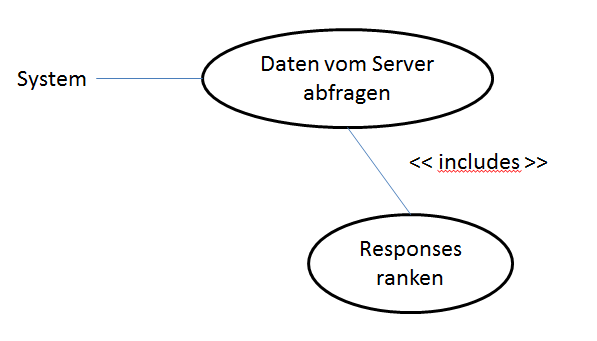
\includegraphics[width=0.6\textwidth]{use-case}
	\caption{Use Case des Rankings}
	\label{fig:Ranking Use-Case}
\end{figure}
\pagebreak